
\begin{frame}[label=basis]
    \frametitle{Basis of Meteor Radar}
    \begin{columns}
        \begin{column}{0.75\textwidth}
            \\ ~ \\ Using ground-based \textbf{\textcolor{blue}{transmitter}}s (\textcolor{blue}{\textbf{TX}}) and \textbf{\textcolor{red}{receiver}}s (\textcolor{red}{\textbf{RX}}):
            \begin{itemize}
                \item Ablating \textbf{\textcolor{cyan}{meteor trails}} act as reflective atmospheric tracers 
                \item \textcolor{red}{\textbf{RX}} compares the signal sent to the echo received
                \item Meteor and environmental parameters estimated 
            \end{itemize}
            % \hl{\textbf{No other way to \textit{densely} sample this region}} 
            \centering
            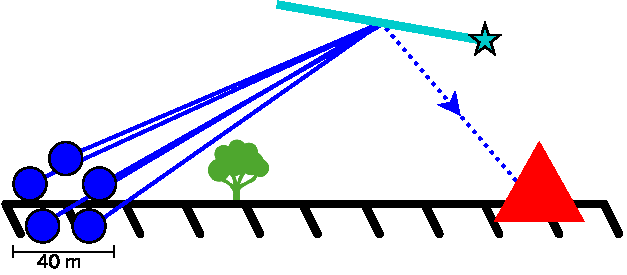
\includegraphics[width=0.85\textwidth]{img/IF_basis.pdf}
            % \begin{tikzpicture}
            %     \node[anchor=south west, inner sep=0] (image) at (0,0) {%
            %     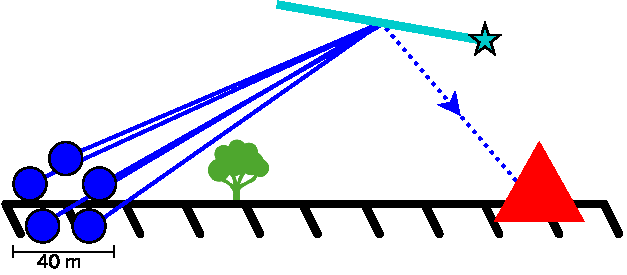
\includegraphics[width=0.85\textwidth]{img/IF_basis.pdf}};
            %     % \node<1->[circle, draw=yellow, fill=yellow!30, thick, minimum size=4mm] at ([xshift=1.05cm, yshift=0.5cm]image.west) {1};
            %     % \uncover<2->{\node[circle, draw=yellow, fill=yellow!30, thick, minimum size=4mm] 
            %     % at ([xshift=0.95cm, yshift=-1.1cm]image.north) {2};}
            %     % \uncover<3->{\node[circle, draw=yellow, fill=yellow!30, thick, minimum size=4mm] 
            %     % at ([xshift=-1.3cm, yshift=0.5cm]image.east) {3};}
            % \end{tikzpicture}
        \end{column}
        % \vrule{}
        \begin{column}{0.3\textwidth}
            \vspace{-10pt}
            \begin{center}%
                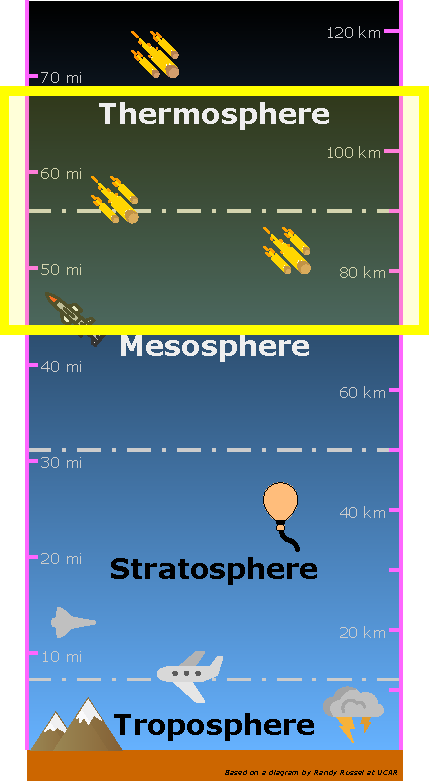
\includegraphics[height=0.65\textheight]{img/atmos_layers.pdf}
            \end{center}
            \footnotesize \vspace{-10pt}
            % \uncover<+->{Ultimate goal: \alert{Science!}
            % \begin{itemize} \scriptsize
            %     \item Seasonal trends
            %     \item Energy transport 
            %     \item Inform atmospheric models 
            % \end{itemize}}
        \end{column}
    \end{columns}
\end{frame}